%%%%%%%%%%%%
%
% $Autor: Wings $
% $Datum: 2019-03-05 08:03:15Z $
% $Pfad: PythonPackages/Contents/General/PixelLib $
% $Version: 4250 $
% !TeX spellcheck = en_GB/de_DE
% !TeX encoding = utf8
% !TeX root = filename 
% !TeX TXS-program:bibliography = txs:///biber
%
%%%%%%%%%%%%



\chapter{Package \PYTHON{PixelLib}}

\section{Introduction}

PixelLib is a Python package specifically crafted to facilitate image and video segmentation within the domain of computer vision. Image segmentation, a pivotal task in computer vision, involves the partitioning of an image into discernible segments or regions based on specific characteristics such as color, texture, or spatial relationships. This segmentation process is crucial for tasks like object recognition, scene understanding, and overall visual content analysis.

By leveraging PixelLib, developers and researchers can streamline and expedite the segmentation process, making it more accessible for various applications. The library's capabilities extend to both images and videos, allowing for comprehensive segmentation analysis in dynamic visual scenarios. With PixelLib, intricate computer vision tasks become more manageable, providing a valuable tool for extracting meaningful insights from visual data.

\section{Detailed Description}
PixelLib supports two major types of segmentation:

\begin{itemize}
    \item \textbf{Semantic Segmentation:} This involves labeling each pixel in an image with a class of what is being represented. Pixels that are part of the same object type get the same label. PixelLib makes semantic segmentation accessible, with support for various pre-trained models.
    
    \item \textbf{Instance Segmentation:} Unlike semantic segmentation, instance segmentation not only labels each pixel of the image but also differentiates between different instances of the same class. This is particularly useful in scenarios where the distinction between individual objects of the same type is crucial.\newline
    
    Furthermore, PixelLib can also be used for background editing in images and videos.
    
    PixelLib supports two deep learning libraries for image segmentation which are Pytorch and Tensorflow.
\end{itemize}

\section{PixelLib Pytorch Version}

The pytorch version of PixelLib uses PointRend object segmentation architecture to replace Mask R-CNN for performing instance segmentation of objects. PointRend is an excellent state of the art neural network for implementing object segmentation. It generates accurate segmentation masks and run at high inference speed that matches the increasing demand for an accurate and real time computer vision applications. PixelLib is a library built to provide support for different operating systems.The PointRend implementation used for PixelLib supports both Linux and Windows OS.

\begin{figure}[h!]
    \centering
    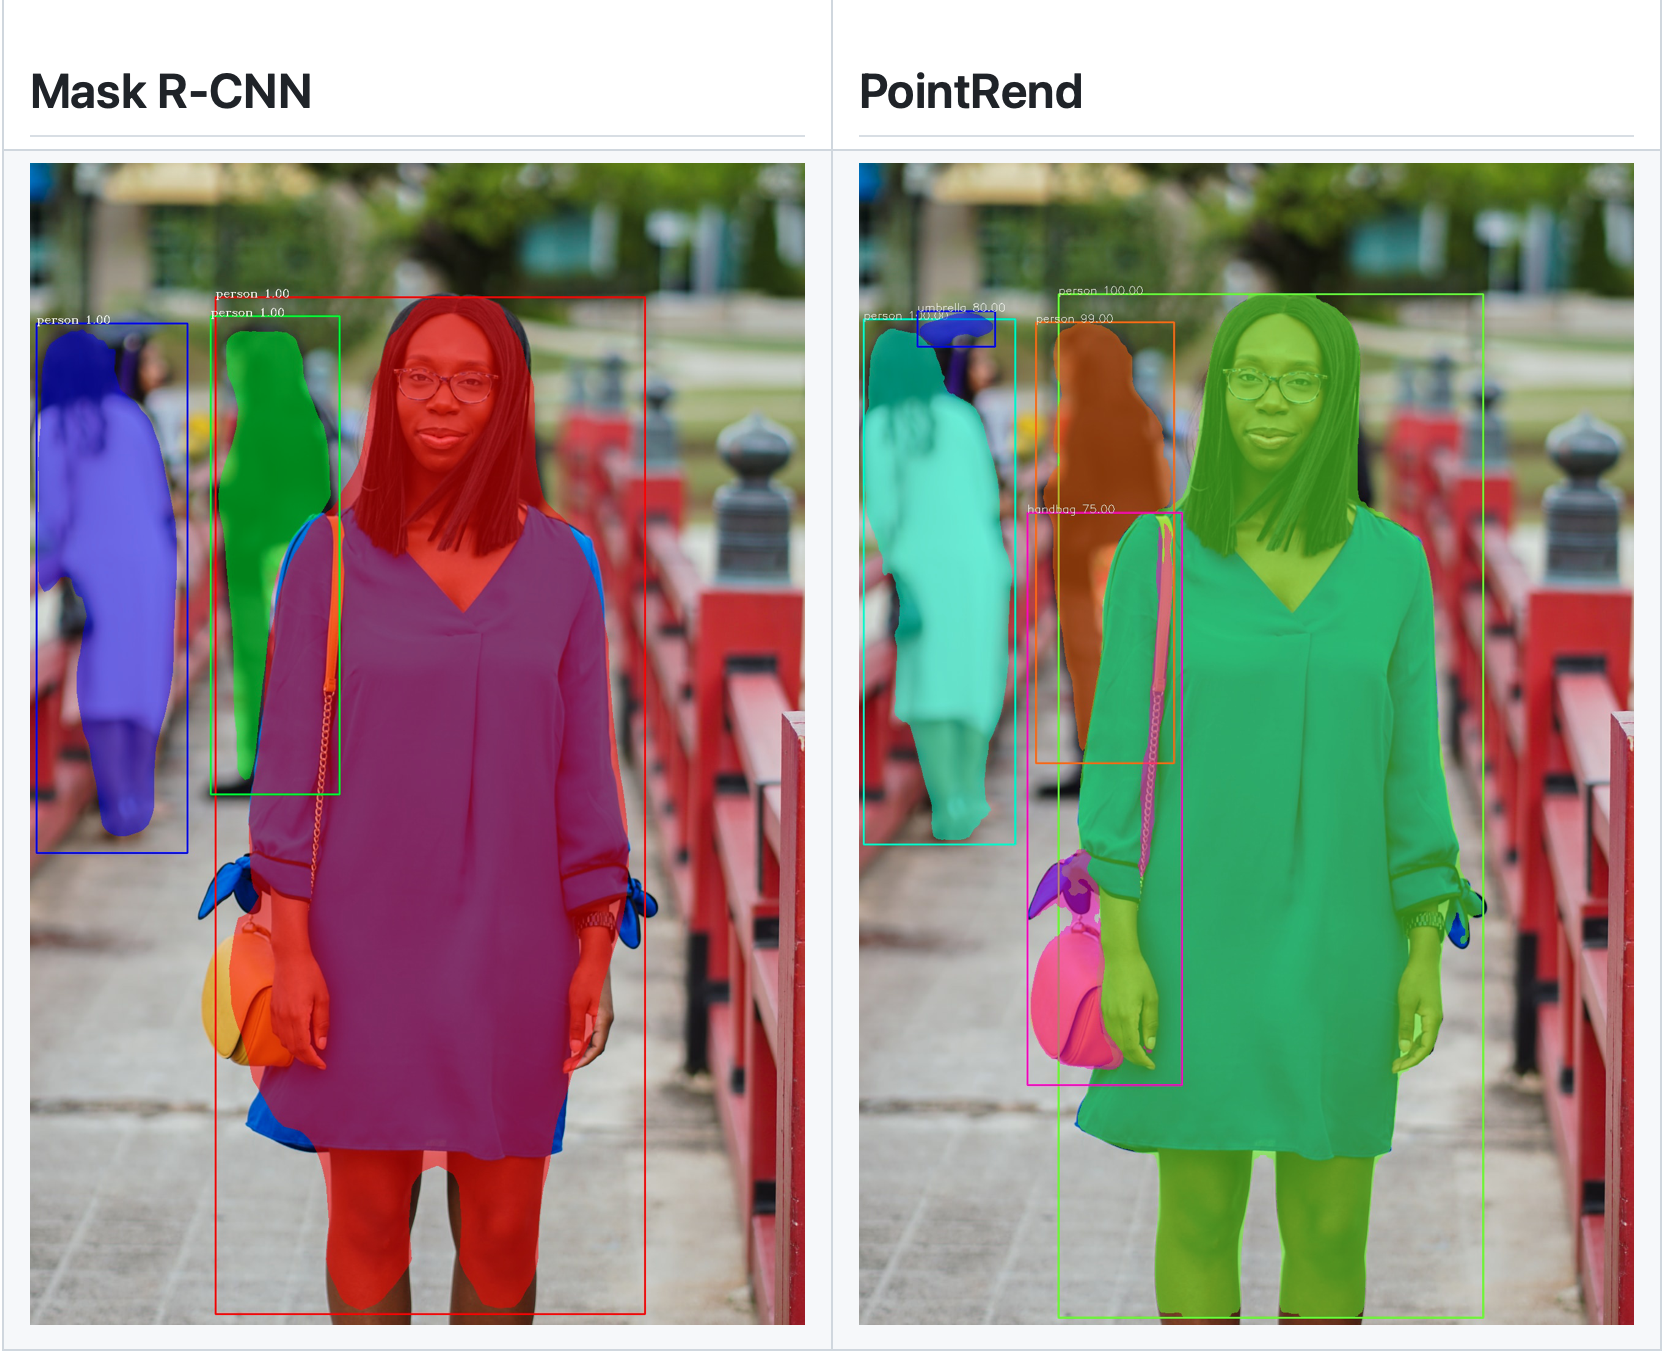
\includegraphics[width=0.8\linewidth]{Images/PixelLib/pytorch1.png} % Adjust the path accordingly
    
    \caption{Mask R-CNN vs PointRend}
    \label{fig:your_image_label}
    
    
\end{figure}

\begin{figure}[h!]
    \centering
    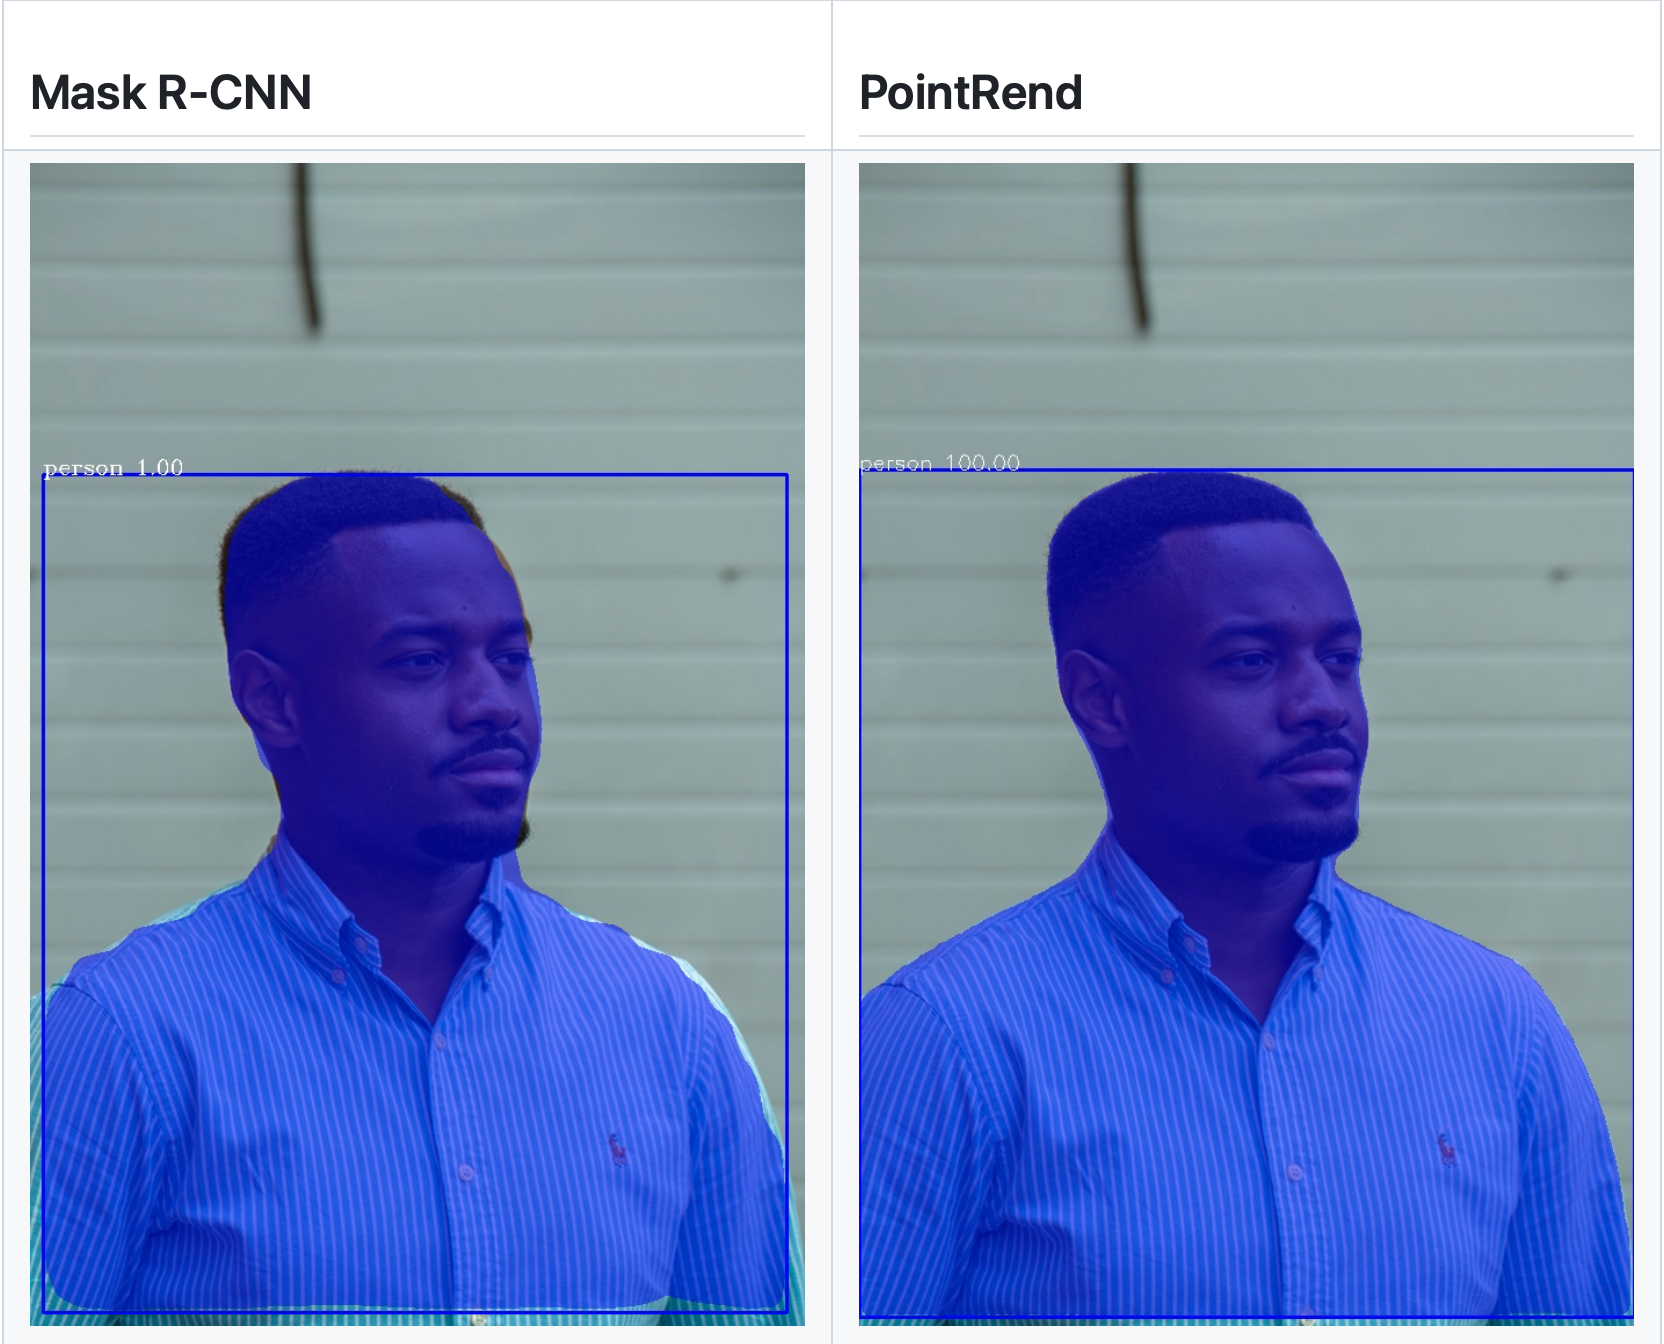
\includegraphics[width=0.8\linewidth]{Images/PixelLib/pytorch2.png} % Adjust the path accordingly
    
    \caption{Mask R-CNN vs PointRend}
    \label{fig:your_image_label}
    
    
\end{figure}


The sample images above are examples of the differences in the segmentation results of PointRend compared to Mask RCNN. It is obvious that the PointRend image results are better segmentation outputs compared to Mask R-CNN results.

\section{Install PixelLib and its dependencies}

Download Python
PixelLib pytorch version supports python version 3.7 and above. Download a \url{https://www.python.org}.\newline


\textbf{Install Pytorch}\newline
PixelLib Pytorch version supports these versions of pytorch(1.6.0, 1.7.1,1.8.0 and 1.9.0).
Note: Pytorch 1.7.0 is not supported and do not use any pytorch version less than 1.6.0. Install a compatible\url{https://pytorch.org}

\textbf{Install Pycocotools}
\begin{verbatim}
    pip3 install pycocotools
\end{verbatim}

\textbf{Install PixelLib}
\begin{verbatim}
    pip3 install pixellib
\end{verbatim}	

If installed, upgrade to the latest version using:
\begin{verbatim}
    pip3 install pixellib — upgrade
\end{verbatim}		

\section{Examples of Semantic Image Segmentation}
PixelLib makes it possible to perform state of the art semantic segmentation of 150 classes of objects with Ade20k model using 5 Lines of Code. Perform indoor and outdoor segmentation of scenes with PixelLib by using Ade20k model.
\begin{figure}[h!]
    \centering
    \includegraphics[width=0.8\linewidth]{Images/PixelLib/sem3.jpg} % Adjust the path accordingly
    
    \caption{Semantic Image Segmentation}
    \label{fig:your_image_label}
    
    
\end{figure}



\subsection{Example Manual}

Semantic Segmentation with Pixellib

\subsection{Description}
This example demonstrates how to use the Pixellib library for semantic segmentation of images using a pre-trained ADE20K model.

\subsection{Files}

\begin{itemize}
    \item \texttt{segmentation\_example.py}: Python script containing the code snippet.
    \item \texttt{deeplabv3\_xception65\_ade20k.h5}: Pre-trained ADE20K model.
    \item \texttt{sample.jpg}: Input image for semantic segmentation.
    \item \texttt{image\_new.jpg}: Output image with segmentation overlay.
\end{itemize}

\subsection{Version}

PixelLib semantic image segmentation supports Python 3.6 and above.

\subsection*{Supported Python Versions}

\begin{itemize}[label=--]
    \item \textbf{TensorFlow version:} PixelLib's TensorFlow version works with Python 3.6 and above.
    \item \textbf{PyTorch version:} This version also supports Python 3.7 and above.
\end{itemize}

\textbf{No additional PyTorch version constraints:} Unlike video segmentation, PyTorch version compatibility is not an issue for image segmentation. As long as you have Python 3.7 or above, you can use any supported PyTorch version.

\subsection*{Choosing the Right Version}

\begin{itemize}[label=--]
    \item \textbf{TensorFlow vs. PyTorch:} Both versions offer semantic image segmentation. Choose TensorFlow if you prioritize ease of use and have existing TensorFlow experience. Otherwise, PyTorch may offer more flexibility and customization.
\end{itemize}

\subsection*{Additional Resources}

\begin{itemize}[label=--]
    \item PixelLib GitHub repository: \url{https://github.com/ayoolaolafenwa/PixelLib}
    \item PixelLib official documentation: \url{https://pixellib.readthedocs.io/en/stable/}
    \item Real-Time Image Segmentation Using 5 Lines of Code: \url{https://towardsdatascience.com/tagged/image-segmentation}
\end{itemize}

\subsection{Example Code}

\begin{lstlisting}[language=Python]
    import pixellib
    from pixellib.semantic import semantic_segmentation
    
    # Create an instance of the semantic_segmentation class
    segment_image = semantic_segmentation()
    
    # Load a pre-trained ADE20K model (DeepLabV3 with Xception65 backbone)
    segment_image.load_ade20k_model("deeplabv3_xception65_ade20k.h5")
    
    # Perform semantic segmentation on the input image "sample.jpg"
    # Overlay the segmentation results on the original image and save as "image_new.jpg"
    segment_image.segmentAsAde20k("sample.jpg", overlay=True, output_image_name="image_new.jpg")
\end{lstlisting}


\subsection*{Code Description of Semantic Image Segmentation}

\textbf{Library and Module Import:}
\begin{itemize}
    \item \texttt{import pixellib:} Imports the \texttt{pixellib} library, which is a Python library for image and video segmentation tasks.
    \item \texttt{from pixellib.semantic import semantic\_segmentation:} Imports the \texttt{semantic\_segmentation} class from the \texttt{pixellib.semantic} module. This class is designed for performing semantic segmentation.
\end{itemize}

\textbf{Instance Creation:}
\begin{itemize}
    \item \texttt{segment\_image = semantic\_segmentation():} Creates an instance named \texttt{segment\_image} of the \texttt{semantic\_segmentation} class. This instance will be used to perform semantic segmentation on images.
\end{itemize}

\textbf{Model Loading:}
\begin{itemize}
    \item \texttt{segment\_image.load\_ade20k\_model("deeplabv3\_xception65\_ade20k.h5"):} Loads a pre-trained semantic segmentation model trained on the ADE20K dataset. The model is based on the DeepLabV3 architecture with the Xception65 backbone.
\end{itemize}

\textbf{Image Segmentation:}
\begin{itemize}
    \item \texttt{segment\_image.segmentAsAde20k("sample.jpg", overlay=True, output\_image\_name="image\_new.jpg"):} Performs semantic segmentation on the input image \texttt{"sample.jpg"} using the loaded ADE20K model. The segmentation results are overlaid on the original image if \texttt{overlay=True}. The processed image is then saved as \texttt{"image\_new.jpg"}.
\end{itemize}

\begin{figure}[h!]
    \centering
    \includegraphics[width=0.8\linewidth]{Images/PixelLib/a5.jpg} % Adjust the path accordingly
    
    \caption{Result of Semantic Image Segmentation}
    \label{fig:your_image_label}
    
    
\end{figure}

\section{Example of Semantic Video Segmentation}

\subsection{Example Manual}
Semantic Segmentation of Videos with Pixellib

\subsection{Description}
This example manual provides instructions on performing semantic segmentation on videos using the Pixellib library with a pre-trained ADE20K model. Semantic segmentation in videos involves labeling each pixel in every frame of the video with a corresponding class label, such as "road," "building," "sky," etc. The example demonstrates how to load the pre-trained model, process a video, and generate an output video with segmentation overlay on each frame.

\subsection{Example Files}
\begin{itemize}
    \item \texttt{semantic\_segmentation\_example.py}: Python script containing the code snippet.
    \item \texttt{deeplabv3\_xception65\_ade20k.h5}: Pre-trained ADE20K model.
    \item \texttt{sample\_video.mp4}: Sample input video for semantic segmentation.
    \item \texttt{output\_video.mp4}: Output video with segmentation overlay.
\end{itemize}

\subsection{Version}
PixelLib semantic video segmentation supports Python 3.7 and above.

\subsection*{PixelLib Versions}
\begin{itemize}[label=--]
    \item \textbf{TensorFlow version:} This version does not support video segmentation.
    \item \textbf{PyTorch version:} This version supports Python 3.7 and above, but requires compatible PyTorch versions:
    \begin{itemize}[label=$\bullet$]
        \item Supported versions: 1.6.0, 1.7.1, 1.8.0, and 1.9.0
        \item Unsupported version: 1.7.0 (avoid using)
        \item Versions less than 1.6.0: Not supported
    \end{itemize}
\end{itemize}

\subsection*{Choosing the Right Version}
\begin{itemize}[label=--]
    \item If you prioritize ease of use and minimal configuration, consider the TensorFlow version (not available for videos).
    \item If you need video segmentation and have more control over your environment, choose the PyTorch version and ensure compatibility with your PyTorch installation.
\end{itemize}

\subsection*{Additional Resources}
\begin{itemize}[label=--]
    \item PixelLib GitHub repository: \url{https://github.com/ayoolaolafenwa/PixelLib}
    \item PixelLib official documentation: \url{https://pixellib.readthedocs.io/en/stable/}
    \item Video segmentation with PixelLib (5 lines of code): \url{https://towardsdatascience.com/tagged/image-segmentation}
\end{itemize}

\subsection{Example Code}
\begin{lstlisting}[language=Python]
    import pixellib
    from pixellib.semantic import semantic_segmentation
    
    # Create an instance of the semantic_segmentation class for video processing
    segment_video = semantic_segmentation()
    
    # Load a pre-trained ADE20K model (DeepLabV3 with Xception65 backbone)
    segment_video.load_ade20k_model("deeplabv3_xception65_ade20k.h5")
    
    # Process a video named "sample_video.mp4" using ADE20K semantic segmentation
    # Overlay the segmentation results on each frame, display at 15 frames per second, and save as "output_video.mp4"
    segment_video.process_video_ade20k("sample_video.mp4", overlay=True, frames_per_second=15, output_video_name="output_video.mp4")
    
    
\end{lstlisting}


\subsection*{Code Description of Semantic Image Segmentation}




\textbf{Library Import:}
\begin{itemize}
    \item \texttt{import pixellib:} Imports the \texttt{pixellib} library, a Python library for image and video segmentation tasks.
    \item \texttt{from pixellib.semantic import semantic\_segmentation:} Imports the \texttt{semantic\_segmentation} class from the \texttt{pixellib.semantic} module. This class is designed for semantic segmentation tasks.
\end{itemize}

\textbf{Instance Creation:}
\begin{itemize}
    \item \texttt{segment\_video = semantic\_segmentation():} Creates an instance named \texttt{segment\_video} of the \texttt{semantic\_segmentation} class. This instance will be used for processing semantic segmentation on a video.
\end{itemize}

\textbf{Model Loading:}
\begin{itemize}
    \item \texttt{segment\_video.load\_ade20k\_model("deeplabv3\_xception65\_ade20k.h5"):} Loads a pre-trained semantic segmentation model named "deeplabv3\_xception65\_ade20k.h5." This model is trained on the ADE20K dataset and is based on the DeepLabV3 architecture with the Xception65 backbone.
\end{itemize}

\textbf{Video Processing:}
\begin{itemize}
    \item \texttt{segment\_video.process\_video\_ade20k("sample\_video.mp4", overlay=True, frames\_per\_second=15, output\_video\_name="output\_video.mp4"):} Processes a video named "sample\_video.mp4" using the loaded ADE20K model. It performs semantic segmentation on each frame, overlays the segmentation results on the original frames (\texttt{overlay=True}), displays the processed video at 15 frames per second, and saves the output video as "output\_video.mp4."
\end{itemize}
\begin{figure}[h!]
    \centering
    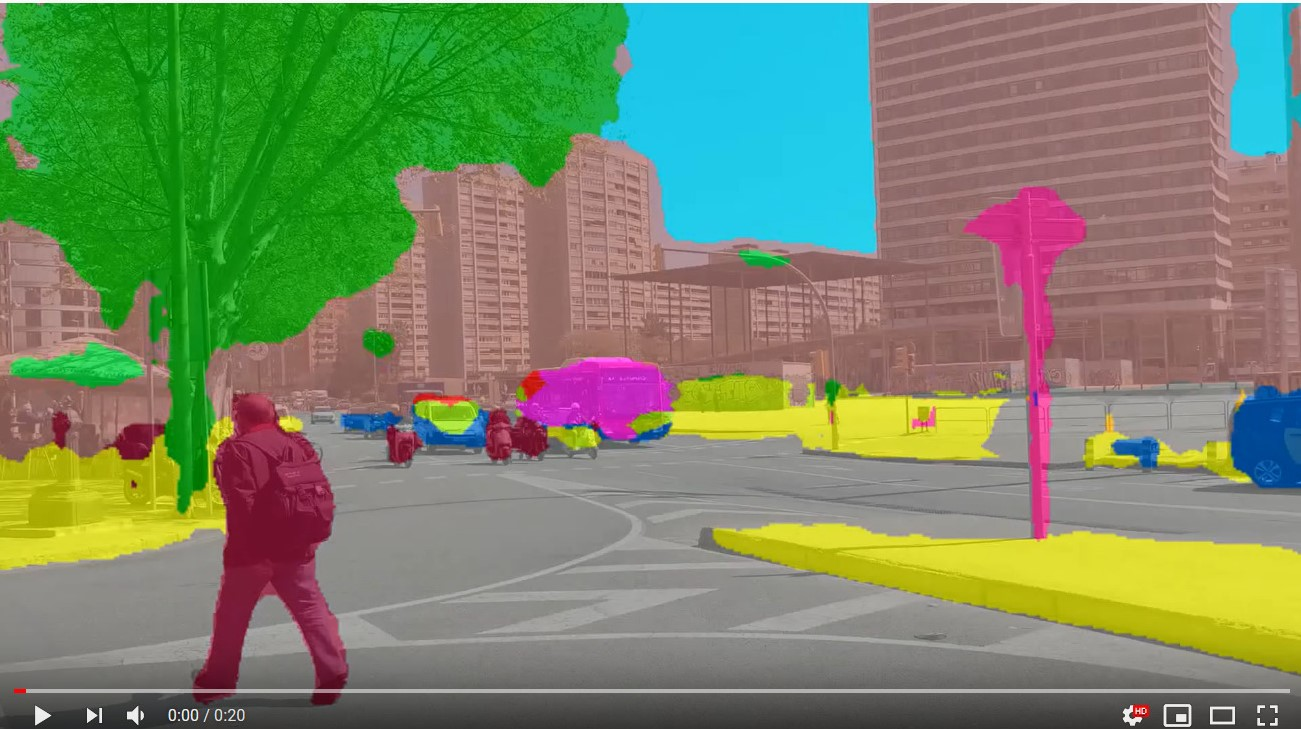
\includegraphics[width=0.8\linewidth]{Images/PixelLib/sem4.jpeg} % Adjust the path accordingly
    
    \caption{Result of Semantic Video Segmentation}
    \label{fig:your_image_label}
\end{figure}


\newpage

\section{Examples of Instance Image Segmentation}


\begin{figure}[h!]
    \centering
    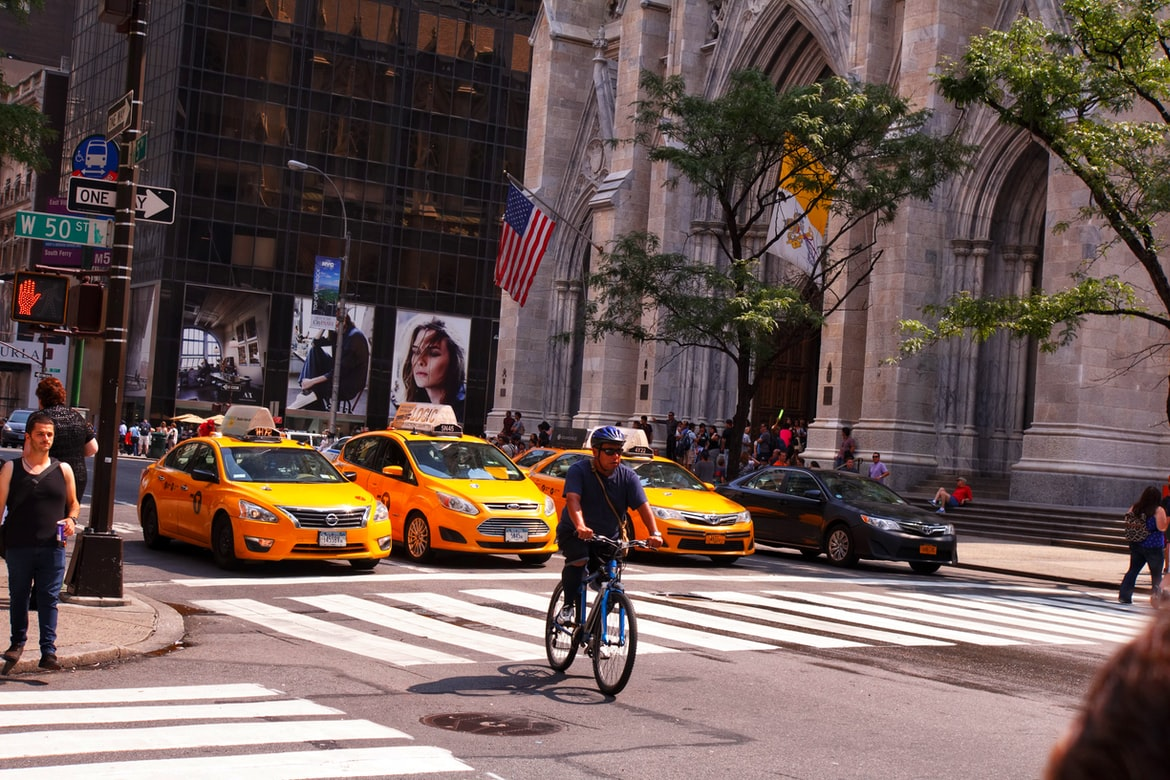
\includegraphics[width=0.8\linewidth]{Images/PixelLib/seg.jpeg} % Adjust the path accordingly
    
    \caption{Image segmentation using PointRed}
    \label{fig:your_image_label}
    
    
\end{figure}
\subsection{Example Manual}
Instance Segmentation with Pixellib

\subsection{Description}
This example manual provides instructions on performing instance segmentation on images using the Pixellib library with a pre-trained model. Instance segmentation is a computer vision task where objects in an image are not only classified into different classes but also segmented and individually identified. The example demonstrates how to load the pre-trained model, process an input image, and generate an output image with bounding boxes around segmented objects.

\subsection{Example Files}
\begin{itemize}
    \item \texttt{instance\_segmentation\_example.py}: Python script containing the code snippet.
    \item \texttt{pointrend\_resnet50.pkl}: Pre-trained model for instance segmentation.
    \item \texttt{image.jpg}: Sample input image for instance segmentation.
    \item \texttt{output\_image.jpg}: Output image with bounding boxes around segmented objects.
\end{itemize}

\subsection{Version}
Supported Python Versions and Dependencies for PixelLib Instance Image Segmentation

\subsection*{TensorFlow Version}
\begin{itemize}[label=--]
    \item \textbf{Python:} This version supports Python 3.5 and above, but it uses TensorFlow 2.x, so make sure you have a compatible version installed.
\end{itemize}

\subsection*{PyTorch Version}
\begin{itemize}[label=--]
    \item \textbf{Python:} This version supports Python 3.7 and above similar to semantic video segmentation.
    \item \textbf{PyTorch:} Similar to video segmentation, it requires specific PyTorch versions:
    \begin{itemize}[label=$\bullet$]
        \item Supported versions: 1.6.0, 1.7.1, 1.8.0, and 1.9.0
        \item Unsupported version: 1.7.0
        \item Versions less than 1.6.0: Not supported
    \end{itemize}
\end{itemize}

\subsection*{Choosing the Right Version}
\begin{itemize}[label=--]
    \item For simplicity and compatibility with older Python versions, choose the TensorFlow version if you don't need video segmentation.
    \item For faster performance and broader model selection, choose the PyTorch version, but ensure your Python and PyTorch versions are compatible.
\end{itemize}

\subsection*{Additional Resources}
\begin{itemize}[label=--]
    \item PixelLib GitHub repository: \url{https://github.com/ayoolaolafenwa/PixelLib}
    \item PixelLib official documentation: \url{https://pixellib.readthedocs.io/en/stable/}
\end{itemize}

\subsection{Example Code}
\begin{lstlisting}[language=Python]
    import pixellib
    from pixellib.torchbackend.instance import instanceSegmentation
    
    # Create an instance of the instanceSegmentation class
    ins = instanceSegmentation()
    
    # Load a pre-trained model named "pointrend_resnet50.pkl"
    ins.load_model("pointrend_resnet50.pkl")
    
    # Perform instance segmentation on the input image "image.jpg"
    # Show bounding boxes on the segmented objects and save the output as "output_image.jpg"
    ins.segmentImage("image.jpg", show_bboxes=True, output_image_name="output_image.jpg")
\end{lstlisting}




\section*{Code description of Instance Image Segmentation}				
\begin{description}
    \item[Library Import:]
    \begin{itemize}
        \item \texttt{import pixellib:} Imports the \texttt{pixellib} library, a Python library for image and video segmentation tasks.
    \end{itemize}
    
    \item[Module Import:]
    \begin{itemize}
        \item \texttt{from pixellib.torchbackend.instance import instanceSegmentation:} Imports the \texttt{instanceSegmentation} class from the \texttt{pixellib.torchbackend.instance} module. This class is designed for performing instance segmentation using PyTorch.
    \end{itemize}
    
    \item[Instance Creation:]
    \begin{itemize}
        \item \texttt{ins = instanceSegmentation():} Creates an instance named \texttt{ins} of the \texttt{instanceSegmentation} class, initializing an object for performing instance segmentation.
    \end{itemize}
    
    \item[Model Loading:]
    \begin{itemize}
        \item \texttt{ins.load\_model("pointrend\_resnet50.pkl"):} Loads a pre-trained instance segmentation model named "pointrend\_resnet50.pkl." This model is based on the ResNet50 architecture and is designed for identifying and segmenting different instances (objects) within an image.
    \end{itemize}
    
    \item[Instance Segmentation:]
    \begin{itemize}
        \item \texttt{ins.segmentImage("image.jpg", show\_bboxes=True, output\_image\_name="output\_image.jpg"):} Performs instance segmentation on the input image "image.jpg" using the loaded model. It shows bounding boxes around the segmented objects (\texttt{show\_bboxes=True}) and saves the output image as "output\_image.jpg."
    \end{itemize}
\end{description}

\begin{figure}[h!]
    \centering
    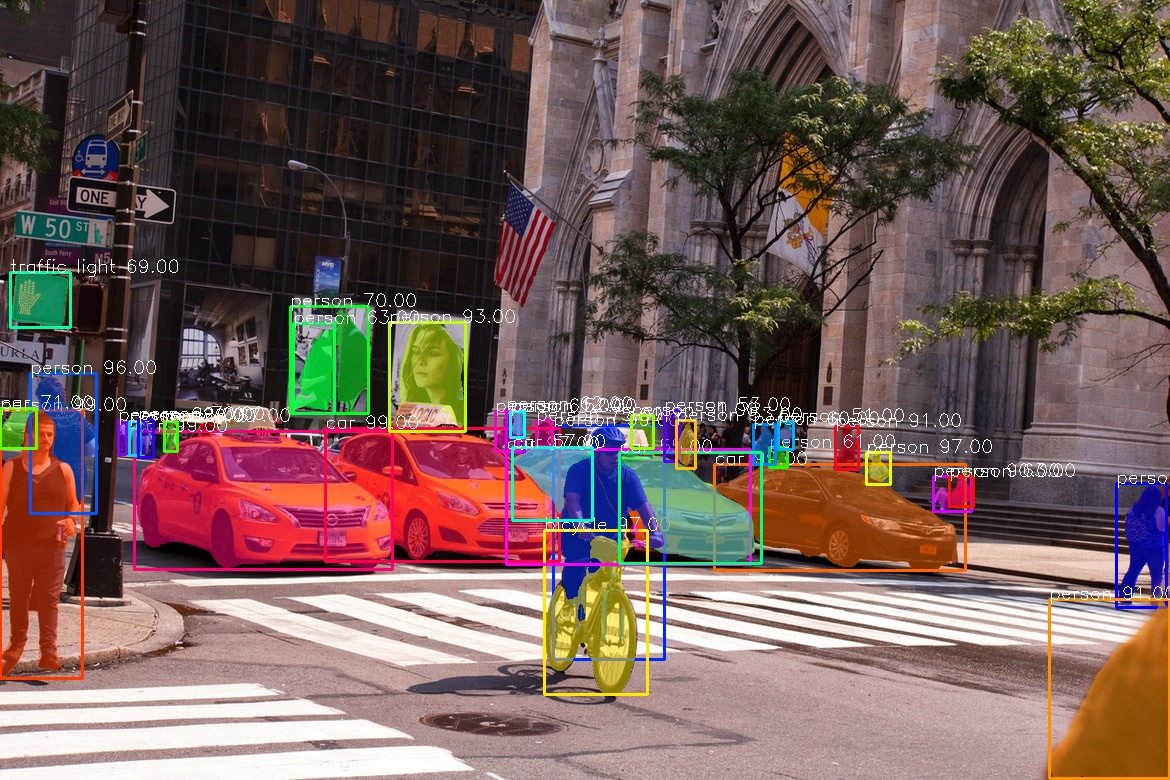
\includegraphics[width=0.8\linewidth]{Images/PixelLib/seg2.jpeg} % Adjust the path accordingly
    
    \caption{Result of Image segmentation using PointRed}
    \label{fig:your_image_label}
    
    
\end{figure}
\newpage		



\section{Example of Instance Video Segmentation}
\subsection{Example Manual}
Instance Video Segmentation with Pixellib
\subsection{Description}
This example manual provides instructions on performing instance segmentation on images and videos using the Pixellib library with a pre-trained model. Instance segmentation is a computer vision task where objects in an image or video are not only classified into different classes but also segmented and individually identified. The example demonstrates how to load the pre-trained model, process input images and videos, and generate output with bounding boxes around segmented objects.

\subsection{Example Files}
\begin{itemize}
    \item \texttt{instance\_segmentation\_image.py}: Python script for image instance segmentation.
    \item \texttt{instance\_segmentation\_video.py}: Python script for video instance segmentation.
    \item \texttt{pointrend\_resnet50.pkl}: Pre-trained model for instance segmentation.
    \item \texttt{sample\_video.mp4}: Sample input video for instance segmentation.
    \item \texttt{image.jpg}: Sample input image for instance segmentation.
    \item \texttt{output\_image.jpg}: Output image with bounding boxes around segmented objects.
    \item \texttt{output\_video.mp4}: Output video with bounding boxes around segmented objects.
\end{itemize}

\subsection{Version}
Compatible Python and PyTorch Versions for PixelLib Instance Video Segmentation

\subsection*{Python Version}
\begin{itemize}[label=--]
    \item Supported: 3.7 and above
\end{itemize}

\subsection*{PyTorch Version}
\begin{itemize}[label=--]
    \item Supported: 1.6.0, 1.8.0, and 1.9.0
    \item Unsupported: 1.7.0 (avoid using)
    \item Versions less than 1.6.0: Not supported
\end{itemize}

\subsection*{Key Points}
\begin{itemize}[label=--]
    \item PixelLib's TensorFlow version does not currently support video segmentation.
    \item Only the PyTorch version offers video segmentation capabilities, including instance segmentation.
    \item Make sure your PyTorch installation aligns with the supported versions mentioned above.
\end{itemize}

\subsection*{Useful Resources}
\begin{itemize}[label=--]
    \item PixelLib GitHub repository: \url{https://github.com/ayoolaolafenwa/PixelLib}
    \item PixelLib official documentation: \url{https://pixellib.readthedocs.io/en/latest/}
    \item Video Segmentation With 5 Lines of Code: \url{https://towardsdatascience.com/video-segmentation-with-5-lines-of-code-87f798afb93}
\end{itemize}

\subsection{Example Code}	
\begin{lstlisting}[language=Python]
    import pixellib
    from pixellib.torchbackend.instance import instanceSegmentation
    
    # Create an instance of the instanceSegmentation class
    ins = instanceSegmentation()
    
    # Load a pre-trained model named "pointrend_resnet50.pkl"
    ins.load_model("pointrend_resnet50.pkl")
    
    # Process a video named "sample_video.mp4"
    # Show bounding boxes on the segmented objects, display 3 frames per second, and save the output as "output_video.mp4"
    ins.process_video("sample_video.mp4", show_bboxes=True, frames_per_second=3, output_video_name="output_video.mp4")
    
\end{lstlisting}


\subsection*{Code description of video segmentation}	
\begin{description}
    \item[Library Import:]
    \begin{itemize}
        \item \texttt{import pixellib:} Imports the \texttt{pixellib} library, a Python library for image and video segmentation tasks.
    \end{itemize}
    
    \item[Module Import:]
    \begin{itemize}
        \item \texttt{from pixellib.torchbackend.instance import instanceSegmentation:} Imports the \texttt{instanceSegmentation} class from the \texttt{pixellib.torchbackend.instance} module. This class is designed for performing instance segmentation using PyTorch.
    \end{itemize}
    
    \item[Instance Creation:]
    \begin{itemize}
        \item \texttt{ins = instanceSegmentation():} Creates an instance named \texttt{ins} of the \texttt{instanceSegmentation} class, initializing an object for performing instance segmentation.
    \end{itemize}
    
    \item[Model Loading:]
    \begin{itemize}
        \item \texttt{ins.load\_model("pointrend\_resnet50.pkl"):} Loads a pre-trained instance segmentation model named "pointrend\_resnet50.pkl." This model is based on the ResNet50 architecture and is designed for identifying and segmenting different instances (objects) within an image.
    \end{itemize}
    
    \item[Video Processing:]
    \begin{itemize}
        \item \texttt{ins.process\_video("sample\_video.mp4", show\_bboxes=True, frames\_per\_second=3, output\_video\_name="output\_video.mp4"):} Processes a video named "sample\_video.mp4." It performs instance segmentation on each frame, shows bounding boxes around the segmented objects (\texttt{show\_bboxes=True}), displays the output at a rate of 3 frames per second, and saves the processed video as "output\_video.mp4."
    \end{itemize}
\end{description}

\begin{figure}[h]
    \centering
    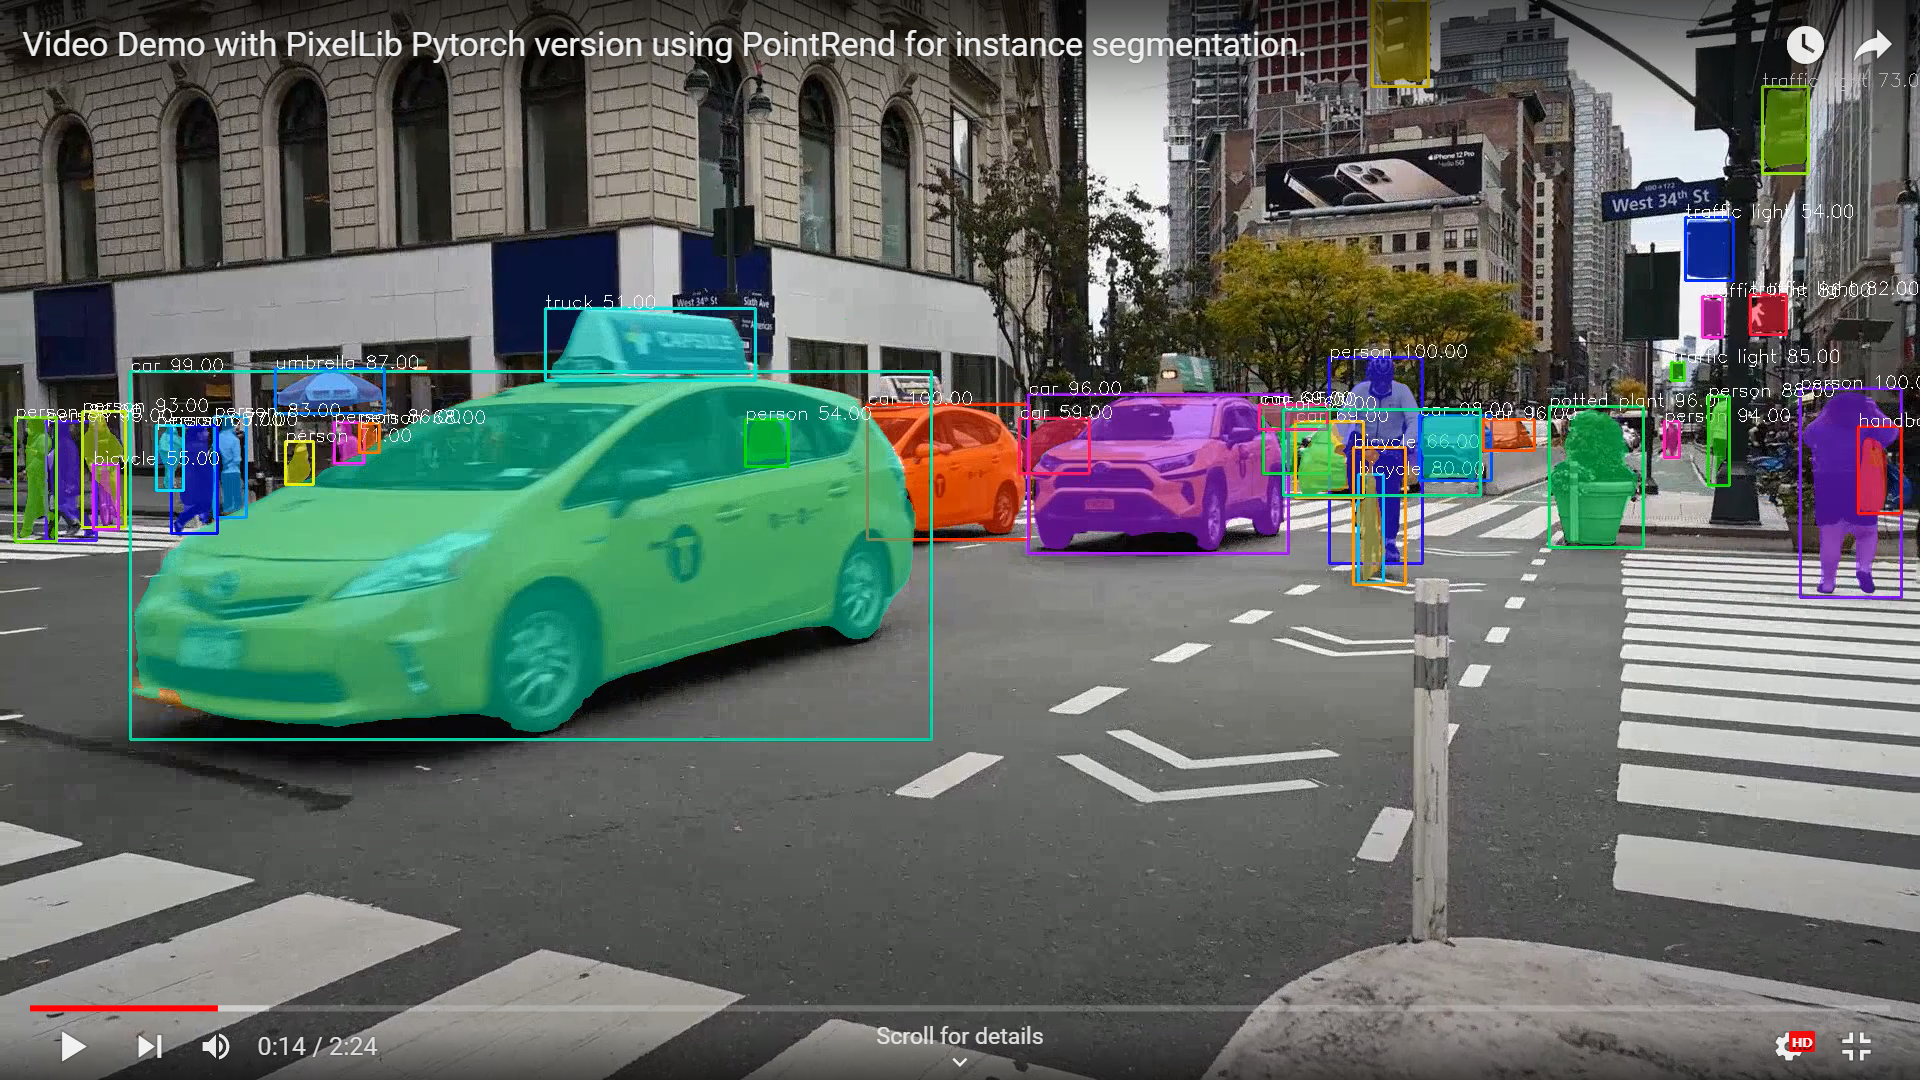
\includegraphics[width=0.8\linewidth]{Images/PixelLib/vid1.png} % Adjust the path accordingly
    
    \caption{Video Segmentation with Pytorch Using PointRend}
    \label{fig:your_image_label}
\end{figure}

\section{Background Editing in Images}




\section*{PixelLib Background Editing Features}

PixelLib uses object segmentation to achieve excellent foreground and background separation, allowing for easy background editing with just five lines of code. The following features are supported:

\subsection*{1. Create a Virtual Background}
Create a virtual background for both images and videos.

\subsection*{2. Assign a Distinct Color to the Background}
Assign a distinct color to the background of both images and videos.

\subsection*{3. Blur the Background}
Blur the background of both images and videos.

\subsection*{4. Grayscale the Background}
Convert the background to grayscale for both images and videos.

\begin{figure}[h!]
    \centering
    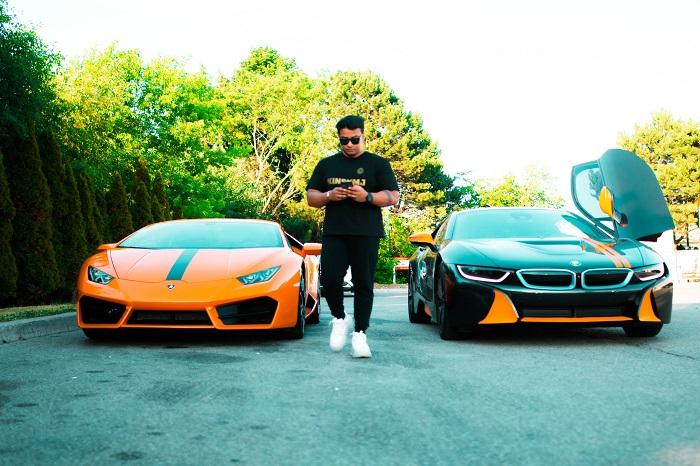
\includegraphics[width=0.8\linewidth]{Images/PixelLib/image5.jpeg} % Adjust the path accordingly
    
    \caption{Image for Background Editing}
    \label{fig:your_image_label}
\end{figure}

\subsection{Example Manual:}
Background  Image Editing with Pixellib


\subsection{Description}
This example manual provides instructions on performing background editing on images using the Pixellib library with a pre-trained model. Background editing is a computer vision task where the background of an image is modified while preserving the foreground objects. The example demonstrates how to load the pre-trained model, apply background editing techniques, and generate output images with modified backgrounds.

\subsection{Example Files}
\begin{itemize}
    \item \texttt{background\_editing.py}: Python script for background editing.
    \item \texttt{xception\_pascalvoc.pb}: Pre-trained model for background editing.
    \item \texttt{sample.jpg}: Sample input image for background editing.
    \item \texttt{blur\_img.jpg}: Output image with background blur.
\end{itemize}

\subsection{Version}
Python Version Support for Background Editing in Images Using PixelLib

\subsection*{PixelLib Versions}
\begin{itemize}[label=--]
    \item \textbf{TensorFlow version:} This version supports Python versions 3.7 and above and is generally easier to set up, but does not support video segmentation.
    \item \textbf{PyTorch version:} This version also supports Python 3.7 and above, but with additional compatibility requirements:
    \begin{itemize}[label=$\bullet$]
        \item Supported PyTorch versions: 1.6.0, 1.7.1, 1.8.0, and 1.9.0
        \item Unsupported version: 1.7.0 (avoid using)
        \item Versions less than 1.6.0: Not supported
    \end{itemize}
\end{itemize}

\subsection*{Choosing the Right Version}
\begin{itemize}[label=--]
    \item \textbf{Prioritize ease of use:} Choose the TensorFlow version if you prefer simpler setup and don't need video segmentation.
    \item \textbf{More control and video support:} Select the PyTorch version if you prefer fine-grained control and require video segmentation features, but remember to ensure compatibility with your PyTorch installation.
\end{itemize}

\subsection*{Additional Notes}
\begin{itemize}[label=--]
    \item The latest version of PixelLib is always recommended for its updated features and bug fixes. You can upgrade using \texttt{pip3 install pixellib --upgrade}.
    \item For more details and specific instructions on installation and usage, refer to the official PixelLib documentation: \url{https://pixellib.readthedocs.io/en/stable/}
\end{itemize}

\subsection{Example Code}
\begin{lstlisting}[language=Python]
    import pixellib
    from pixellib.tune_bg import alter_bg
    
    # Create an instance of the alter_bg class for background editing
    change_bg = alter_bg(model_type="pb")
    
    # Load a pre-trained Pascal VOC model based on Xception architecture
    change_bg.load_pascalvoc_model("xception_pascalvoc.pb")
    
    # Apply extreme blur to the background of the input image "sample.jpg"
    # Only blur the region where a person is detected in the image
    # Save the output as "blur_img.jpg"
    change_bg.blur_bg("sample.jpg", extreme=True, detect="person", output_image_name="blur_img.jpg")
    
    
\end{lstlisting}


\subsection*{Code Description of Image background editing}

\textbf{Library and Module Import:}
\begin{itemize}
    \item \texttt{import pixellib:} Imports the \texttt{pixellib} library, a Python library for image and video segmentation tasks.
    \item \texttt{from pixellib.tune\_bg import alter\_bg:} Imports the \texttt{alter\_bg} class from the \texttt{pixellib.tune\_bg} module. This class is designed for background editing.
\end{itemize}

\textbf{Instance Creation:}
\begin{itemize}
    \item \texttt{change\_bg = alter\_bg(model\_type="pb"):} Creates an instance named \texttt{change\_bg} of the \texttt{alter\_bg} class for background editing. The \texttt{model\_type="pb"} specifies the model type to be used.
\end{itemize}

\textbf{Model Loading:}
\begin{itemize}
    \item \texttt{change\_bg.load\_pascalvoc\_model("xception\_pascalvoc.pb"):} Loads a pre-trained Pascal VOC model based on the Xception architecture. This model is used for background editing.
\end{itemize}

\textbf{Background Editing - Blur Operation:}
\begin{itemize}
    \item \texttt{change\_bg.blur\_bg("sample.jpg", extreme=True, detect="person", output\_image\_name="blur\_img.jpg"):} Applies extreme blur to the background of the input image \texttt{"sample.jpg."} The blur operation is performed selectively only on the region where a person is detected in the image. The processed image is saved as \texttt{"blur\_img.jpg."}
\end{itemize}

\begin{figure}[h!]
    \centering
    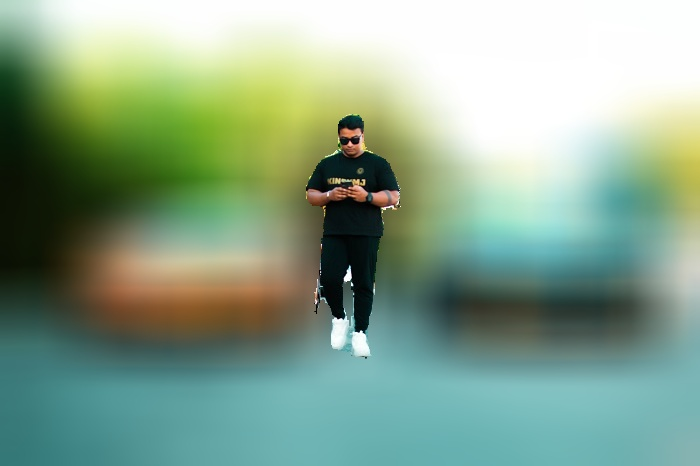
\includegraphics[width=0.8\linewidth]{Images/PixelLib/blur_person.jpg} % Adjust the path accordingly
    
    \caption{Blur Background Image}
    \label{fig:your_image_label}
\end{figure}
\newpage

\section{Background Editing in Videos}
\subsection{Example Manual:}
Video Background Editing with Pixellib

\subsection{Description}
This example manual provides instructions on performing video background editing using the Pixellib library with a pre-trained model. Video background editing involves changing the background of a video while preserving the foreground objects. The example demonstrates how to load the pre-trained model, apply background editing techniques to a video, and generate an output video with the background changed.

\subsection{Example Files}
\begin{itemize}
    \item \texttt{background\_editing.py}: Python script for video background editing.
    \item \texttt{xception\_pascalvoc.pb}: Pre-trained model for background editing.
    \item \texttt{sample\_video.mp4}: Sample input video for background editing.
    \item \texttt{bg.jpg}: Background image to replace the original background.
    \item \texttt{output\_video.mp4}: Output video with background change applied.
\end{itemize}

\subsection{Version}
PixelLib Support for Background Editing in Videos

PixelLib supports background editing in videos for Python versions 3.7 and above, regardless of whether you choose the TensorFlow or PyTorch version. The distinction with PyTorch lies in video segmentation:

\subsection*{PyTorch Version}
\begin{itemize}[label=--]
    \item Offers both background editing and video segmentation functionalities.
    \item Requires compatible PyTorch versions (1.6.0, 1.7.1, 1.8.0, 1.9.0). Skip 1.7.0 and avoid versions below 1.6.0.
\end{itemize}

\subsection*{TensorFlow Version}
\begin{itemize}[label=--]
    \item Provides background editing but not video segmentation.
    \item Generally easier to install and configure but lacks segmentation capabilities.
\end{itemize}

Therefore, depending on your goal:

\begin{itemize}[label=--]
    \item \textbf{For background editing only:} Either TensorFlow or PyTorch versions work with Python 3.7+. Choose TensorFlow for simplicity but remember its limitations.
    \item \textbf{For both background editing and video segmentation:} Go with the PyTorch version with compatible PyTorch installations.
\end{itemize}

\subsection*{Additional Notes}
\begin{itemize}[label=--]
    \item The official PixelLib documentation and repository clearly state support for background editing across both versions:
    \begin{itemize}[label=$\bullet$]
        \item \url{https://pixellib.readthedocs.io/en/stable/}
        \item \url{https://github.com/ayoolaolafenwa/PixelLib}
    \end{itemize}
\end{itemize}

\subsection{Example Code}
\begin{lstlisting}[language=Python]
    import pixellib
    from pixellib.tune_bg import alter_bg
    
    # Create an instance of the alter_bg class for video background editing
    change_bg = alter_bg(model_type="pb")
    
    # Load a pre-trained Pascal VOC model based on the Xception architecture
    change_bg.load_pascalvoc_model("xception_pascalvoc.pb")
    
    # Change the background of the input video "sample_video.mp4" using the background image "bg.jpg"
    # Process the video at a rate of 10 frames per second
    # Save the output as "output_video.mp4" with background change applied selectively on the detected person
    change_bg.change_video_bg("sample_video.mp4", "bg.jpg", frames_per_second=10, output_video_name="output_video.mp4", detect="person")
    
\end{lstlisting}


\subsection*{Code Description of background Video Editing}

\textbf{Library and Module Import:}
\begin{itemize}
    \item \texttt{import pixellib:} Imports the \texttt{pixellib} library, a Python library for image and video segmentation tasks.
    \item \texttt{from pixellib.tune\_bg import alter\_bg:} Imports the \texttt{alter\_bg} class from the \texttt{pixellib.tune\_bg} module. This class is designed for video background editing.
\end{itemize}

\textbf{Instance Creation:}
\begin{itemize}
    \item \texttt{change\_bg = alter\_bg(model\_type="pb"):} Creates an instance named \texttt{change\_bg} of the \texttt{alter\_bg} class for video background editing. The \texttt{model\_type="pb"} specifies the model type to be used.
\end{itemize}

\textbf{Model Loading:}
\begin{itemize}
    \item \texttt{change\_bg.load\_pascalvoc\_model("xception\_pascalvoc.pb"):} Loads a pre-trained Pascal VOC model based on the Xception architecture. This model is used for video background editing.
\end{itemize}

\textbf{Video Background Editing:}
\begin{itemize}
    \item \texttt{change\_bg.change\_video\_bg("sample\_video.mp4", "bg.jpg", frames\_per\_second=10, output\_video\_name="output\_video.mp4", detect="person"):} Changes the background of the input video \texttt{"sample\_video.mp4"} using the background image \texttt{"bg.jpg."} The video is processed at a rate of 10 frames per second, and the output is saved as \texttt{"output\_video.mp4"} with the background change applied selectively on the detected person.
\end{itemize}
\begin{figure}[h!]
    \centering
    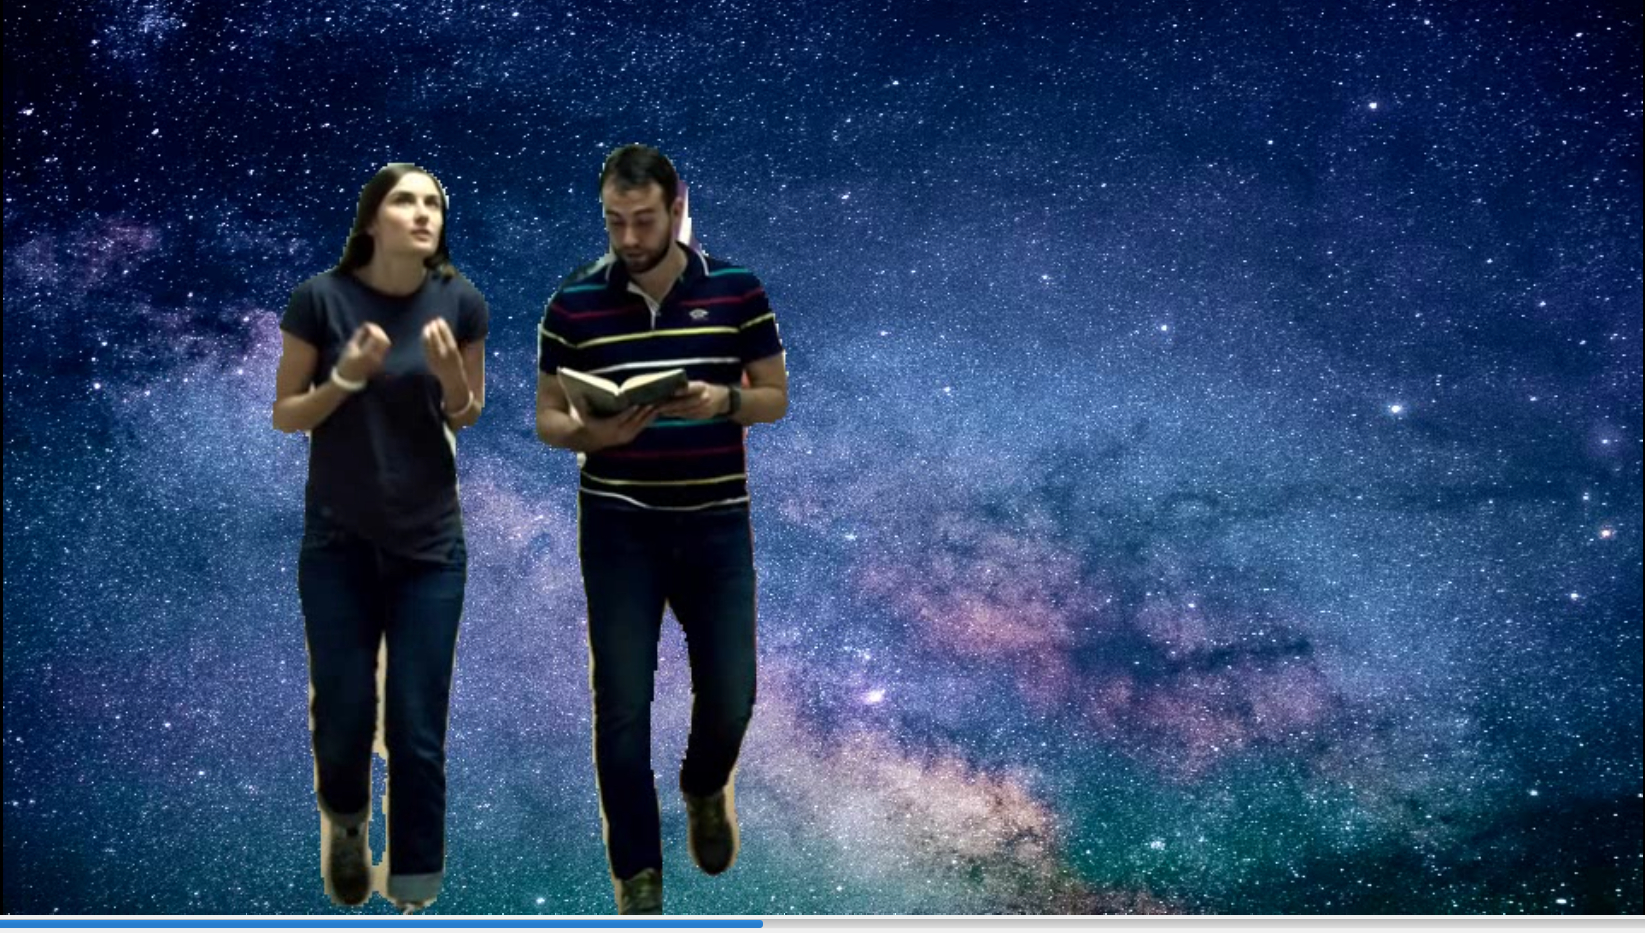
\includegraphics[width=0.8\linewidth]{Images/PixelLib/video2.png} % Adjust the path accordingly
    
    \caption{Edited Background Video}
    \label{fig:your_image_label}
\end{figure}





\section{Further Reading}
For more in-depth information, tutorials, and community support, the following resources are invaluable:

\begin{itemize}
    \item PixelLib's Official Documentation: Offers comprehensive details on installation, API usage, and examples. Visit \url{https://pixellib.readthedocs.io/en/latest/}.
    
    \item GitHub Repository: For the latest updates, issues, and contributions from the developer community. Visit PixelLib on GitHub: \url{https://github.com/ayoolaolafenwa/PixelLib}.
    
    \item PyPI Page: Provides information on the latest releases, project history, and download files. Visit PixelLib on PyPI: \url{https://libraries.io/pypi/pixellib}.
\end{itemize}

PixelLib stands as a user-friendly and powerful tool for image and video segmentation, making it easier for developers and researchers to implement complex segmentation tasks in their projects.


